\scanpage{5}
\mspage{2}
(which is probably always true, and \deleted{in} the criterion for a non-wildness of $\gamma$) we are reduced to the preceding case, by \deleted{removing} replacing $Y'$ by $Y'\setminus S'$, where $S'$ is the finite set of ramification points for the action of $\gamma$. \deleted{\unsure{$E$}}

One should note that the \deleted{condition} \inserted{property} under consideration \deleted{is not} (on the automorphisms of finite order of the surface $Y'$) is not satisfied without restriction. If for example $Y'=\mathbb{C}^*$, or $Y'=\mathbb{U}\times\mathbb{U}$ then translations by points of finite order are isotopic to the identity, without necessarily being equal to the identity ! But we have this
\figure{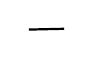
\begin{tikzpicture}[baseline=0pt]\draw[line width=.8pt] (0,0)--(.45,.01);\end{tikzpicture}}

\uline{Proposition 2} Let $Y'$ be an \uline{anabelian} oriented surface of finite type (compact \inserted{surface} $-$ finite number of points), i.e. such that for every connected component $Y'_i$ of $Y'$, we have $\chi_!(Y'_i)<0$ (i.e. we have $2g_i+\nu_i\geq 3$, where $g_i$ is the genus of $Y'_i$ and $\nu_i$ the number of holes\ldots). Then every automorphism \inserted{$\gamma$} of finite order of $Y'_i$ which is isotopic to the identity is the identity.

As $\gamma$ leaves the connected components invariant, we may assume $Y'$ connected. In fact, it suffices that $\gamma$ act trivially on the homology \inserted{$H_1$} (\inserted{for example} with coefficients in $\mathbb{Z}$, or in \inserted{a} $\mathbb{Z}/n\mathbb{Z}$ with $n\geq3$) for
\margin{4}
